% !TEX encoding = UTF-8 Unicode

\documentclass[a4paper]{article}

\usepackage{color}
\usepackage{url}
%\usepackage[T2A]{fontenc} % enable Cyrillic fonts
\usepackage[utf8]{inputenc} % make weird characters work
\usepackage{graphicx}
\usepackage{caption}
\usepackage{subcaption}
\usepackage[english,serbian]{babel}
%\usepackage[english,serbianc]{babel} %ukljuciti babel sa ovim opcijama, umesto gornjim, ukoliko se koristi cirilica
\setcounter{tocdepth}{1}
\usepackage[unicode]{hyperref}
\hypersetup{colorlinks,citecolor=green,filecolor=green,linkcolor=blue,urlcolor=blue}
\usepackage{amsmath}
%\newtheorem{primer}{Пример}[section] %ćirilični primer
\newtheorem{primer}{Primer}[section]
\newtheorem{definicija}[primer]{Definicija}
\captionsetup[figure]{name=Grafik}
\graphicspath{{./images/}}

\begin{document}

\title{Analiza podataka o globalnom terorizmu \\ \small{~\\Seminarski rad u okviru kursa\\Istraživanje podataka\\ Matematički fakultet}}

\author{
	Una Stanković, Uroš Stegić\\
	una\_stankovic@yahoo.com, mi10287@alas.matf.bg.ac.rs}
\date{16.~maj 2017.}
\maketitle


\tableofcontents

\newpage


\section{Uvod}
\label{sec:uvod}
Terorizam je pojam koji se u poslednjih 50 godina sve češće javlja,a posebno u formi globalni terorizam, zato što je terorizam pojava koja je zahvatila ceo svet. U radu će biti predstavljena analiza baze podataka, otvorenog koda, o globalnom terorizmu, dobijena primenom metoda i tehnika obrađenih na kursu Istraživanje podataka.\\\\ 
\subsection{Terorizam}
Prema jednoj od definicija \textit{terorizam je smišljena upotreba nezakonitog nasilja ili pretnje nasiljem radi usađivanja straha, sa namerom prisiljavanja ili zastrašivanja vlasti ili društva, kako bi se postigli najčešće politički verski ili ideološki ciljevi.} \\\\
Posmatrajući globalni nivo, ne postoji nijedna država na svetu koja je imuna na terorizam. On je poput bolesti koja počne iz jednog centra, a potom se širi na sve veće i veće oblasti. U početku je terorizam bio motivisan težnjama ka slobodi, borbama za nacionalno oslobođenje, borbi protiv režima, ali, vremenom, terorizam je poprimio nove, mnogo brutalnije i opasnije oblike.\\
Jedna od najvećih opasnosti terorizma, i jedan od razloga zašto je terorizam veoma opaka $"$bolest$"$, leži u tome što on direktno ugrožava unutrašnju i međunarodnu bezbednost, ali kao najgoru posledicu od svih, on ugrožava bezbednost pojedinca. Posmatrajući terorizam makar i u samo poslednjih nekoliko godina, iako on ni po čemu nije novost, jer se, u relativno savremenom obliku, javio još 1950-ih godina, možemo uočiti da je zahvatio ceo svet i da više niko ne može da se oseća apsolutno bezbedno. Teroristima više nisu glavne mete državne zgrade, zvaničnici ili velike kompanije, već su mete što širi dijapazon ljudi, bez obzira na poreklo, profesiju, religiju ili rasu. Poruka koju teroristi današnjice žele da pošalju je - niko nije bezbedan. \\\\
Terorizam ima veliki uticaj u međunarodnim odnosima i ekonomiji, a poslednjih nekoliko godina aktivno utiče na promenu demografske slike Evrope i izaziva kontroverzne i, često, nehumane reakcije mnogih država Evropske unije, kao i stvaranje neonacističkih i ultranacionalističkih pokreta koji se aktivno bore protiv imigranata. Osim ovakvih grupa, aktivan je porast i u broju terorističkih organizacija i njihovih članova, koji popularizacijom, dostupnošću pristupa i anonimnosti na internetu uspevaju da dopru do novih, sve mlađih, članova.\\ Upravo zbog ogromnog uticaja koji terorizam ima na stvaranje novog svetskog poretka veoma je važno vršiti analizu podataka o terorističkim napadima, kako bi se došlo do zaključaka u kom pravcu se terorizam kreće, koliku štetu nanosi, kakve promene donosi, koliko života odnosi i kako će se u budućnosti razvijati, sa ciljem da se budući napadi lakše predvide, preduprede i spreče, ili da se barem broj budućih žrtava svede na minimum.

\subsection{O podacima}
Baza podataka o globalnom terorizmu (engl. The Global Terrorism Database - GTD) je baza otvorenog koda koja uključuje sistematski organizovane podatke koji sadrže informacije o preko 150 000 terorističkih napada, u periodu od 1970. godine do 2015. godine. U okviru baze je sadržano preko stotinu atributa koje se odnose na lokaciju, taktike, mete, ishode i ostale relevantne informacije. Ova baza o internacionalnim terorističkim incidentima se održava od strane istraživača na Univerzitetu u Merilendu (SAD).

\section{Analiza podataka}
\label{sec:analiza}

U ovoj sekciji predstavićemo analizu podataka na osnovu informacija o globalnom terorizmu dobijenih iz baze primenom metoda koji su rađeni na kursu Istraživanje podataka. 

\subsection{Prečišćavanje podataka}

Informacije dobijene u .csv fajlu sadržale su izuzetno veliki skup atributa, što je osnovni razlog da izvršimo prečišćavanje. Prečišćavanje podataka spada u fazu pretprocesiranja podataka, koje podrazumeva pripremu podataka pre same primene metoda istraživanja podataka. Odlučili smo da, zbog velike količine atributa, odbacimo one koji nemaju prevelik uticaj na analizu i bez kojih se vidljivost ponašanja podataka ne gubi.

Postupak koji smo pratili prilikom prečišćavanja:
\begin{enumerate} 
	\item izabrali smo podskup od 13 atributa za koje smatrali da nam mogu biti od koristi: 
	\begin{itemize}
		\item \textbf{id} - numerički atribut, sistem za zapisivanje id-ja događaja se sastoji iz 12 cifara u formatu yyyymmdd gde yyyy označava godinu, mm mesec i dd dan kada se događaj odigrao,
		\item \textbf{year} - numerički atribut, označava godinu u kojoj se incident dogodio, u slučaju da je incident trajao duži vremenski period, uzima se godina prvog događaja,
		\item \textbf{month} - numerički atribut, označava mesec u kojoj se incident dogodio. U slučaju da je incident trajao duži vremenski period, uzima se mesec prvog događaja, a u slučaju da se ne zna tačan mesec početka stavlja se 0,
		\item \textbf{day} - numerički atribut, označava dan u kojoj se incident dogodio. U slučaju da je incident trajao duži vremenski period, uzima se dan prvog događaja, a u slučaju da se ne zna tačan dan početka stavlja se 0,
		\item \textbf{country} - kategorički atribut, označava državu ili lokaciju gde se incident desio,
		\item \textbf{state} - imenski atribut, označava prvu nenacionalnu regiju gde se događaj odigrao,
		\item \textbf{target} - kategorički atribut, označava uopšteni vid mete ili žrtve,
		\item \textbf{attack} - kategorički atribut, označava generalni vid napada i, neretko, širi skup taktika primenjenih pri napadu. Za svaki incident može se sačuvati do 3 taktike.
		\item \textbf{weapon} - kategorički atribut, po incidentu se može sačuvati do 4 vrste oružja korišćenih pri napadu,
		\item \textbf{fatalities} - numerički atribut, označava zvanični broj ljudi koji su izgubili život pri napadu,
		\item \textbf{injuries} - numerički atribut, predstavlja broj potvrđenih povređenih osoba sa obe strane.\\
	\end{itemize}
	Napomena: ulaz u same algoritme cine svi atributi osim atributa koji se odnosi na id. 
\item izbacili smo sve instance koje sadrže nedostajuće vrednosti, nakon čega je ostalo 115 617 instanci,
\item napisali smo skirptu kojom smo imenske atribute koji su bili u teksutalnom obliku preveli u numeričke vrednosti.

\end{enumerate}

\subsection{Korelacija}
  
Podaci su dosta nezavisni, većina atributa nije korelirana, drugim rečima, koeficijent korelacije većine atributa se nalazi u intervalu $($ $-10^{-2}$, $10^{-2}$ $)$ sa najvećom koncentracijom oko nule. Od 66 parova atributa, mi imamo 17 koji su iz tog intervala bez nule, 7 koji su neke značajnije korelacije, a sve ostalo su nule. Od značajnijih korelacija izdvajamo sledeće: 
\begin{itemize} 
	\item godina-longituda (0.52): \\ Naime, sa proticanjem godina teroristički napadi se događaju sve zapadnije.\\ Napomena: postoji i korelacija između godine i latitude i ona iznosi 0.19 
	\item vrsta napada-vrsta oružja (0.52): \\ Ova korelacija je očekivana, jer se za različite vrste napada koriste odgovarajuće vrste oružja, na primer bombaški napad podrazumeva korišćenje bombe ili drugih eksplozivnih sredstava. 
	\item broj povređenih-broj poginulih (0.39) \\ Ovakav odnos se objašnjava time da postoji određena veza između broja povređenih i poginulih. 
	\item vrsta mete - napad (0.2) \\ Očekivano je da se određene mete napadaju odgovarajućom tehnikom napada, na primer besmisleno je razmatrati napad vojnog ili civilnog objekta hladnim oružjem.\\ 
\end{itemize}

Ovom analizom smo došli kako do očekivanih, tako i do neočekivanih korelacija. S obzirom da se veliki broj terorističkih napada u početku odigravao u predelima Indije, Bliskog istoka i istočnih zemalja, iznenađuje korelacija koja nam ukazuje na to da se u poslednjih nekoliko godina ti napadi pomeraju sve zapadnije, prvenstveno ka Evropi i Americi. Ova korelacija nam može biti dosta korisna, u smislu da nam može pomoći pri uočavanju trenda kretanja i predviđanja budućih napada.

\subsection{Analiza raspodele oružja}

Razmotrimo sada raspodelu upotrebljenog oružja od 1970. do 2015. godine. S obzirom na vremenski period koji posmatramo, zarad bolje preglednosti, odabrali smo nekoliko ``prirodnih'' intervala na koje možemo podeliti sledeće periode: 
\begin{itemize}
	\item 1970-1980
	\item 1981-1990
	\item 1991-2000
	\item 2001-2015\\ 
\end{itemize} 
godine.\\
Za svaki period hoćemo da prikažemo sumarnu statistiku zastupljenosti vrste oružja. Posmatrajmo sada grafik \ref{fig:oruzja}. Već na prvi pogled se uočava da je raspodela oružja po periodima na koje smo podelili interval veoma slična. Naime, u napadima se ``tradicionalno'' koriste vatreno oružje i eksplozivi, nešto ređe zapaljivo oružje i borba ``prsa u prsa'', a retko se koriste hemijsko, lažno i ostalo oružje.

\begin{figure}[h!]
\centering
\includegraphics[width=\textwidth]{zastupljenost.png}
\caption{Raspodela zastupljenosti vrsta oružja}
\label{fig:oruzja}
\end{figure} 

\subsection{Klasetovanje}

Na kraju, predstavićemo klaster analizu svih podataka.\\
S obzirom na činjenicu da ne možemo sa sigurnošću odrediti broj klastera i na osnovu činjenice da je skup trening instanci dovoljno gust (u odnosu na dimenzionalnost podataka), odlučili smo da za klasterovanje koristimo DBSCAN.	\\

Ukoliko prilikom klasterovanja zahtevamo veću gustinu (kao što je prikazano na slici \ref{fig:epsmanje}), instance koji se izdvajaju predstavljaju napade koji su se desili u Indiji i na Bliskom istoku, na osnovu čega zaključujemo da nema značajnih razlika među napadima u tim regionima. \\

Ukoliko se zahteva manja gustina (kao što je prikazano na slici \ref{fig:epsvece}), ne mogu se primetiti značajnije pravilnosti, izuzev toga da postoji razlika u napadima po kontinentima, takva da napadi u Evropi i Africi imaju sličniji karakter u odnosu na napade koji su se dogodili u Aziji.\\
   
\begin{figure}
\centering
\begin{subfigure}[h!]{\textwidth}
	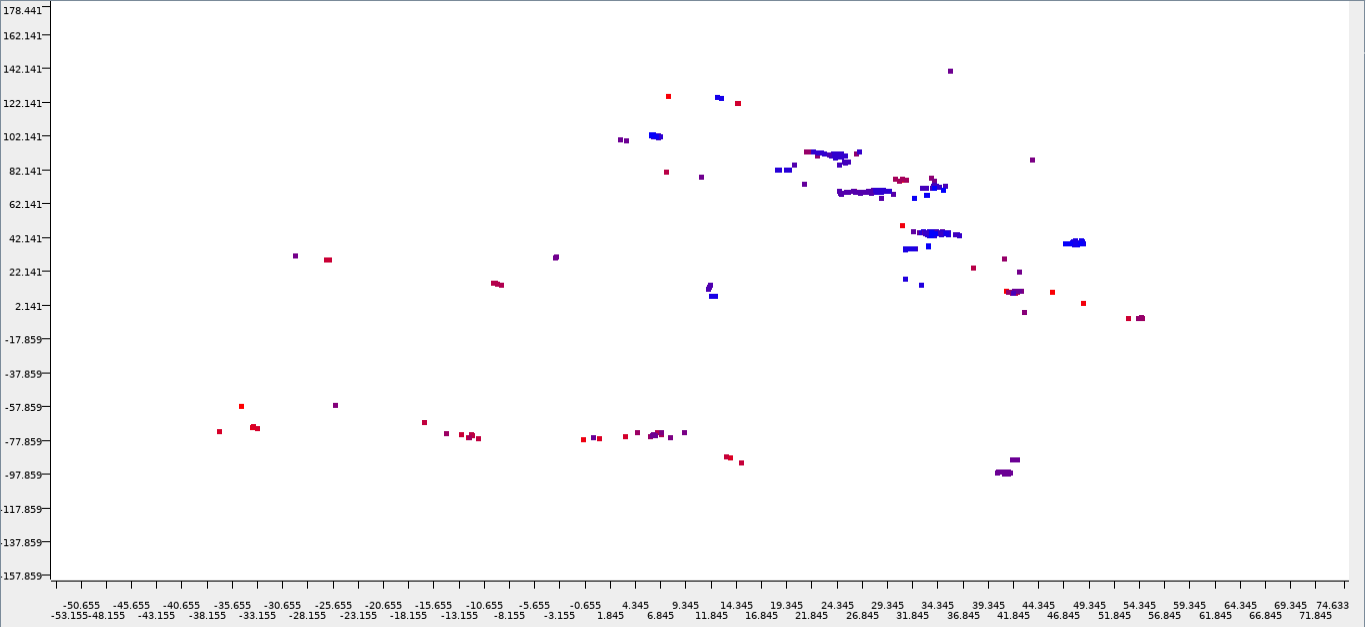
\includegraphics[width=\textwidth]{02_010.png}
	\caption{eps=2, samples=10}
\end{subfigure} 
\begin{subfigure}[h!]{\textwidth}
	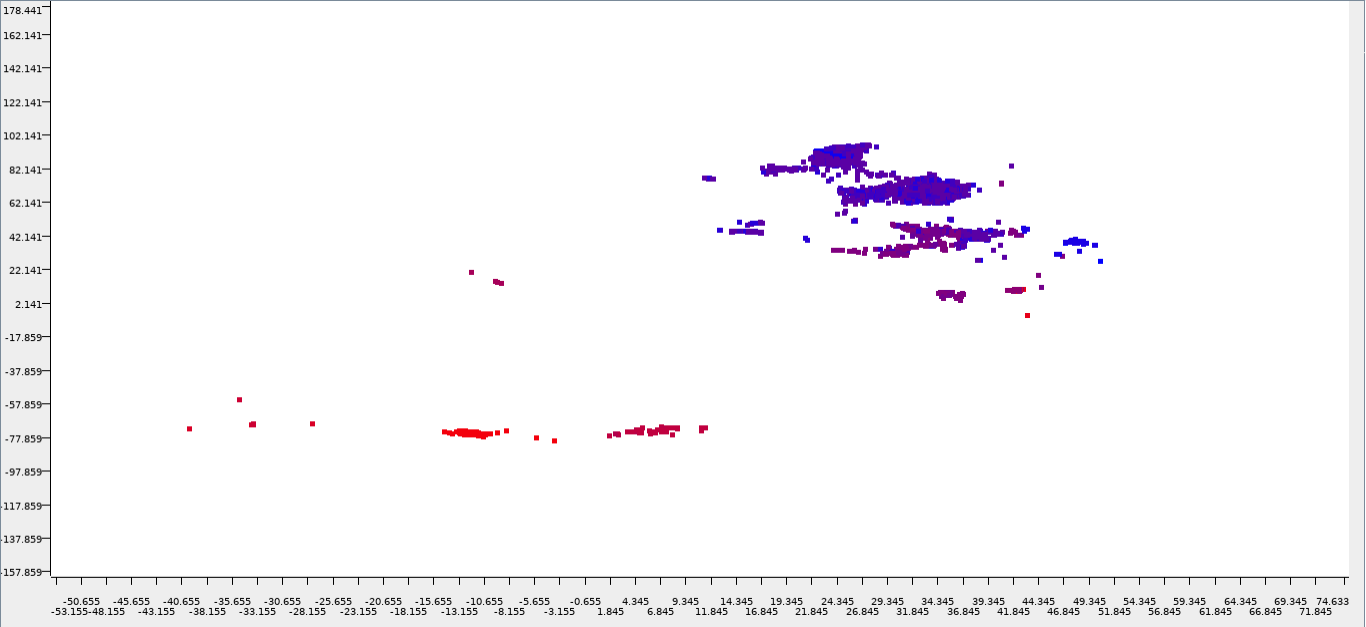
\includegraphics[width=\textwidth]{08_080.png}
	\caption{eps=8, samples=80}
\end{subfigure}
\caption{Tačkasti dijagrami DBSCAN klasterovanja ($eps <= 8$ )}
\label{fig:epsmanje}
\end{figure} 

\begin{figure}
\centering  
\begin{subfigure}[h!]{\textwidth}
	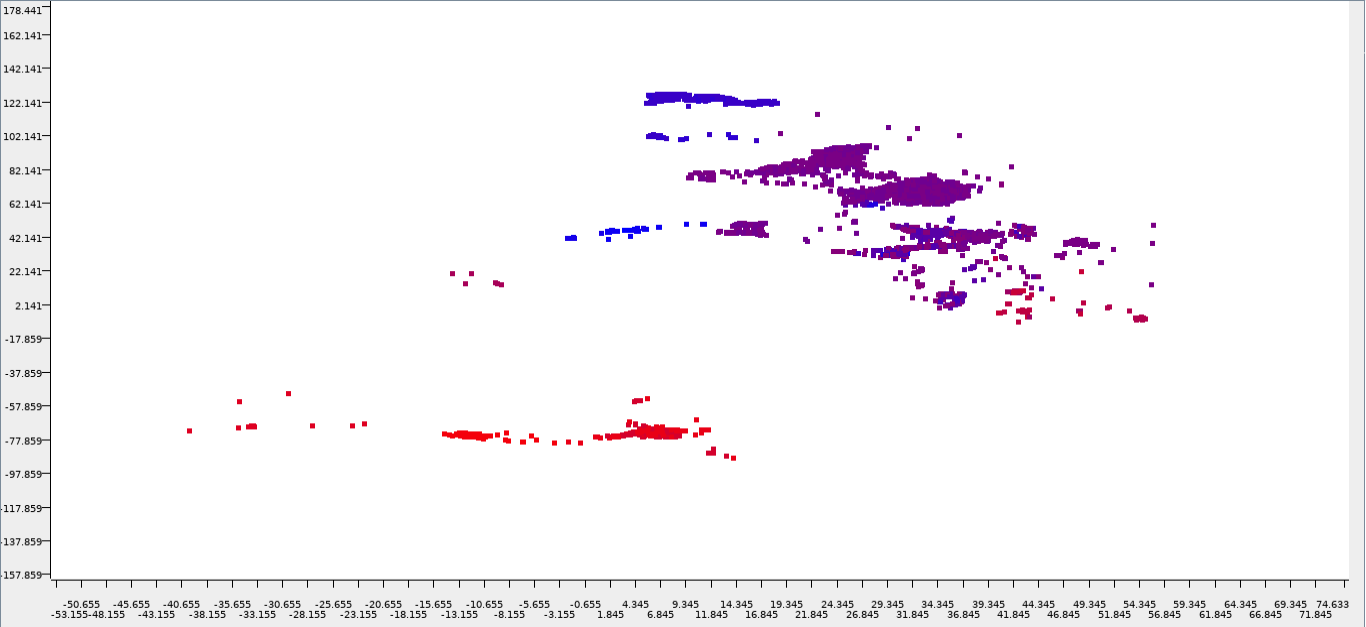
\includegraphics[width=\textwidth]{09_080.png}
	\caption{eps=9, samples=80}
\end{subfigure} 
\begin{subfigure}[h!]{\textwidth}
	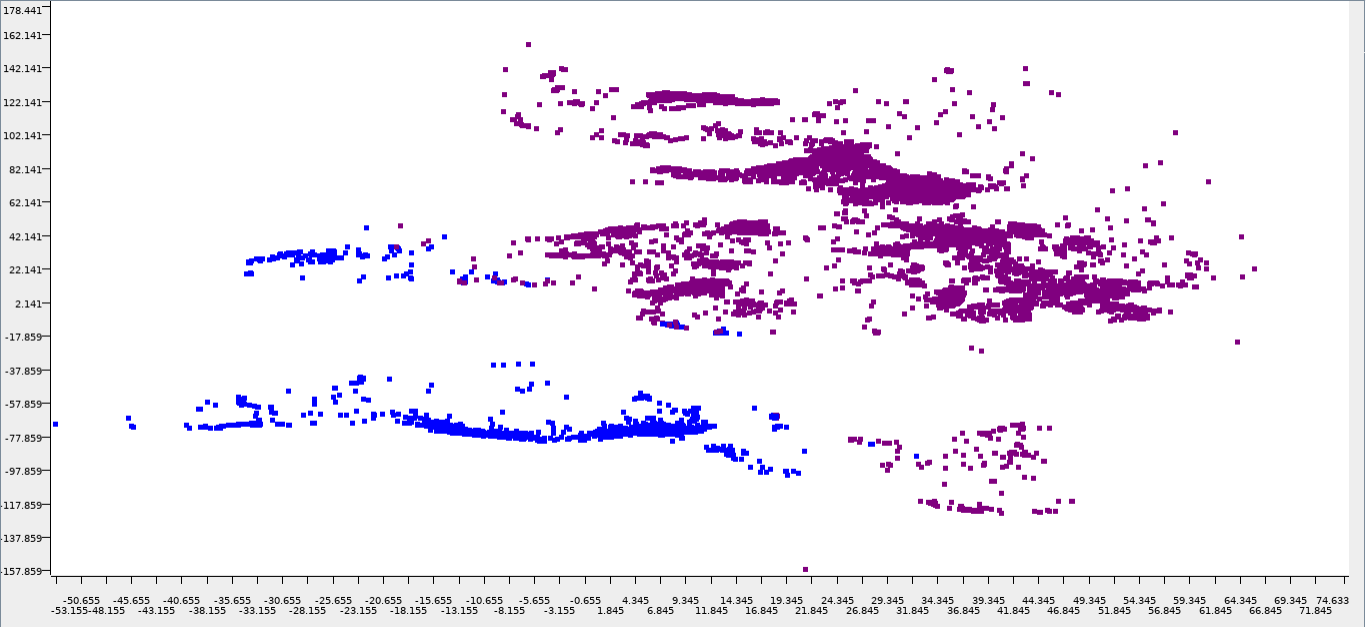
\includegraphics[width=\textwidth]{15_200.png}
	\caption{eps=15, samples=200}
\end{subfigure} 
\caption{Tačkasti dijagrami DBSCAN klasterovanja ($eps > 8$ )}
\label{fig:epsvece}
\end{figure} 


\newpage
\section{Zaključak}
\label{sec:zakljucak}
Na osnovu podataka koje smo dobili analizom, došli smo do sledećih zaključaka:
\begin{itemize}
	\item napadi se kreću ka zapadu,
	\item odnos oružja koje se koristi se ne menja značajno,
	\item napadi koji se dešavaju u Aziji se razlikuju od napada na zapadu.
\end{itemize}
Veliki trud se ulaže u smanjenje globalnog terorizma i nadamo se da će upravo analiza podataka biti od velikog značaja u sprečavanju terorizma u budućnosti i pomoći da se spasu desetine hiljada ljudskih života koji se svake godine ugase isključivo zbog terorizma. Na osnovu prikazanih rezultata, u budućim istraživanjima je moguće izgraditi regresione modele, kojima bi se vršila predikcija manje bezbednih zona i dao uvid u efikasnije mere odbrane od terorizma. 

\end{document}
